\documentclass[a4paper,12pt]{article}
\newcounter{example}[]
\newenvironment{example}[1][]{\refstepcounter{example}\par\medskip
   \noindent \textbf{Example~\theexample. #1} \rmfamily}{\medskip}
   %%%%%%%%%%%%%%%%%%%%%%%%%%%%%%%%

%%%%%%%%%%%%%%%%%%%%%%%%%%%%%%%%%%
\usepackage[utf8]{inputenc}
\usepackage[english]{babel}
\usepackage{tikz-cd}
\usepackage{amsmath,amsfonts,amssymb,amsthm}
\usepackage{mathtools}
 \usepackage{float}
\usepackage{amsthm}
\usepackage{cite}
\usepackage{datetime} % British format dates
\usepackage[cm]{fullpage}
\usepackage{url}
\usepackage{hyperref}
\usepackage{stackrel,amssymb,amsmath}
\usepackage[nottoc]{tocbibind}
\usepackage{pgfplots}
\usepackage{rotating}
\usepackage[autostyle]{csquotes}
\usepackage{natbib}
\usepackage{graphicx}
\usepackage{natbib}
\usepackage{graphicx}

\newtheorem{problem}{Problem}
\newtheorem{attempt}{Attempt}


\newtheorem{theorem}{Theorem}[section]
\newtheorem{corollary}{Corollary}[theorem]
\newtheorem{lemma}[theorem]{Lemma}
\newtheorem{proposition}[theorem]{Proposition}
\theoremstyle{definition}
\newtheorem{definition}{Definition}[section]
\theoremstyle{indented}
\newtheorem*{remark}{Remark}
\newenvironment{titlemize}[1]{%
  \paragraph{#1}
  \begin{itemize}}
  {\end{itemize}}
  
  \usepackage[T1]{fontenc}
\usepackage{imakeidx}
\makeindex[columns=3, title=Alphabetical Index, intoc]
  
  
  %%%%%%%%%%5
\newcommand{\rightarrowdbl}{\rightarrow\mathrel{\mkern-14mu}\rightarrow}

\newcommand{\xrightarrowdbl}[2][]{%
  \xrightarrow[#1]{#2}\mathrel{\mkern-14mu}\rightarrow
}
%%%%%%%%%%%%%%5

\title{Leftovers}
\author{Rhys Wells}
\date{\today}

\begin{document}

\maketitle

\begin{titlemize} {Leftovers list}

  \item Hyperplanes $\sum x_i=k$ give linear functions + intervals. 
      \subitem Linear function: ie $\sum x_i$ gives :$ S \mapsto linear function$ 
       \subitem Value:  and k value gives : $ \text{ value of f on S} \rightarrow \mathbb{Z}$.
       
\item 
\begin{figure}[H]
    \centering
 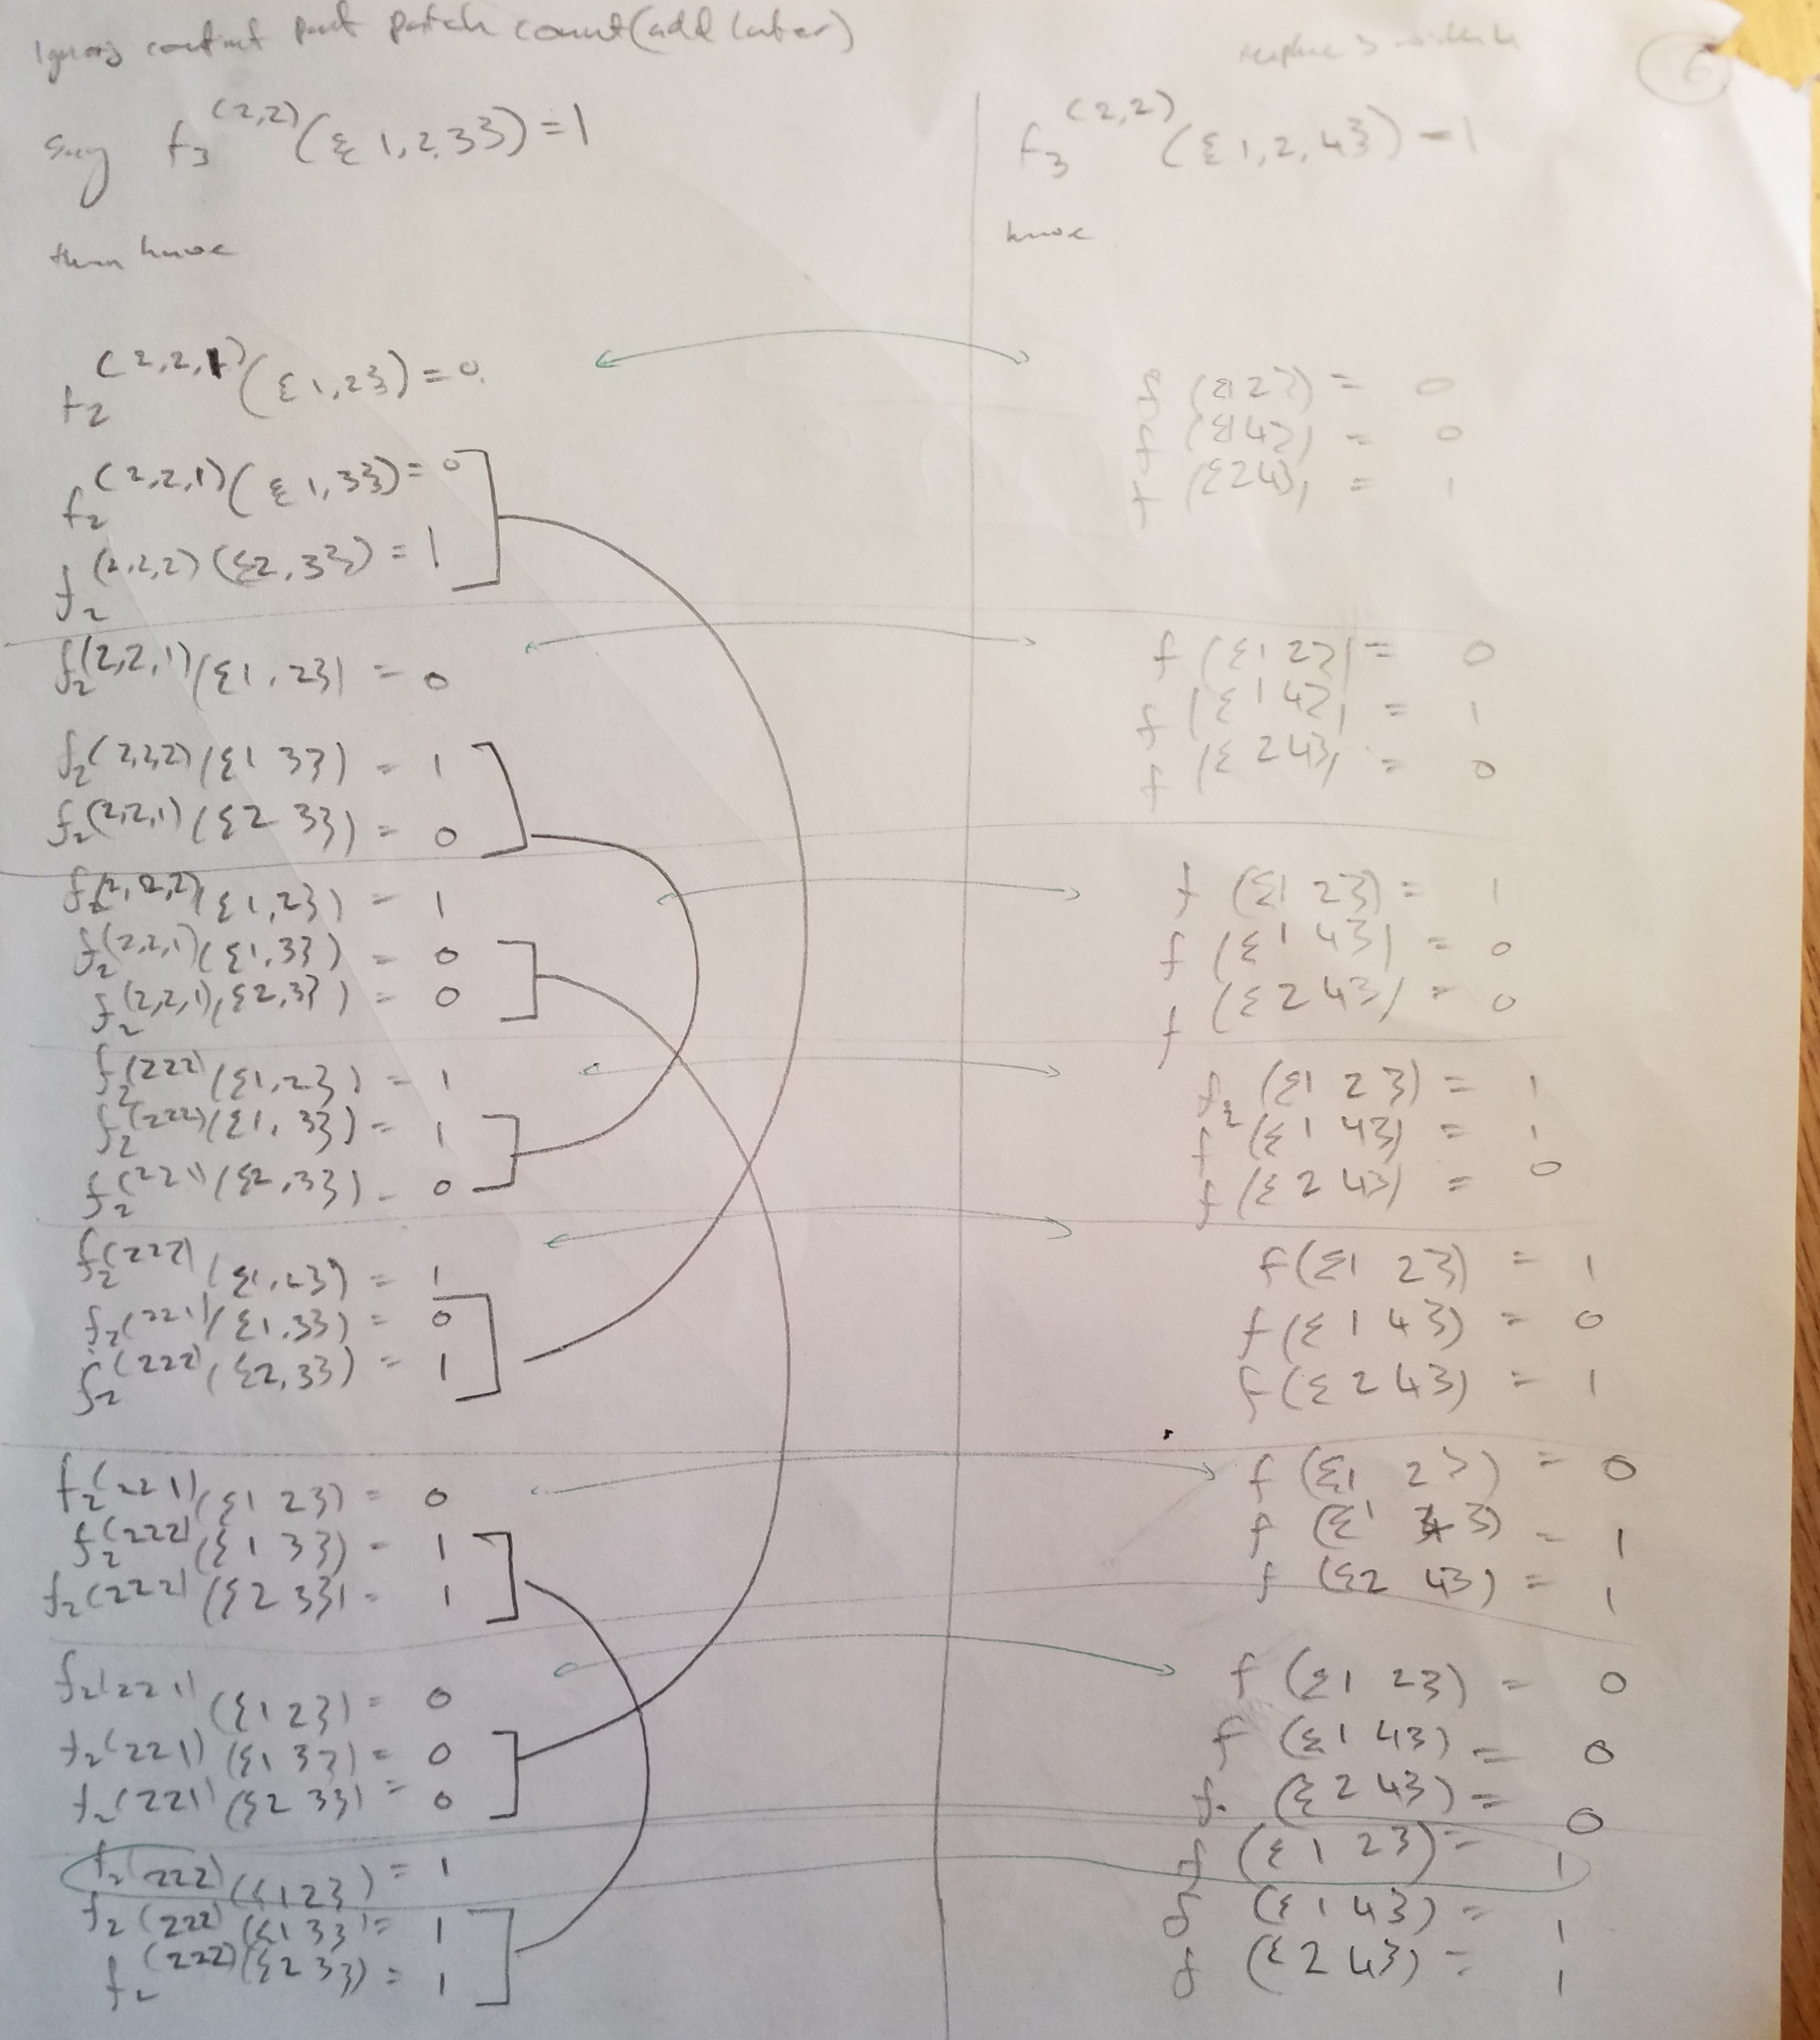
\includegraphics[scale=0.10,angle=0]{29072020 pics/n4level2.jpg}  
    \caption{$n=4$ level 2 values: When $f_3 (I)=1$, I have ignore the index counting the functions}
    \label{}
\end{figure}
\item 
\begin{titlemize} {Notes (this needs correcting)}
\item 

If Nicolas total is correct (the $n=4$ count is $154$). The two corners give $2$ pieces leaving $152$, dividing by $2$ (due to symmetry assuming it work this way) gives $76$. Hence we expect $76$ functions in region $2$ i.e where choices for level $3$ values are either $0$ or $1$.


\item 
After subtracting the $8$ from type $(1,0,0,0)$ combinations of level $3$. We expect $76-8=68$ and this decomposes as $6 \cdot - + 4\cdot - = 68$. By symmetry with $(1,0,0,0)$ I expect the $(1,1,1,0)$ combination of values to give $8$. My gut tells me it decomposes as $6 \cdot 8 + 4\cdot 8 = 68$
\end{titlemize}

\end{titlemize}


\item 
%Going the other way. Give ${}^{i}f^{(2,2)}_{3} (\{1,2,3\})=1$ by n=3 case we have 8 choices for values at level 2. Fixing a choice for e.g $i=1$ e.g $B_1$. Note that in the ${}^{i}f^{(2,2)}_{3} (\{1,2,4\})=1$ case this has the tuple $\{1,2\}$ which already has its value determined earlier. Therefore the free cases are ${}^{1}f^{(2,2,-)}_{2} (\{1,4\})=-$ and ${}^{1}f^{(2,2,-)}_{2} (\{2,4\})=-$ where each can be either $0$ or $1$ (4 options). There is also $\{3,4\}$ which needs to be deterined by either ${}^{i}f^{(2,1)}_{3} (\{1,3,4\})=0$ or ${}^{i}f^{(2,1)}_{3} (\{2,3,4\})=0$.



\section{Supplementary notes for me}

\begin{titlemize}{Possible notation}
    \item  Define $\mathbb{Z}^{ 2^{[n]} \setminus \{\emptyset\} } := \{ f : 2^{[n]} \setminus \{\emptyset\} \rightarrow \mathbb{Z} \} $. 
\end{titlemize}
 
 

  Given a function of the form $f:2^{[n]} \rightarrow \mathbb{Z}$ we recall that element of $2^{n}$ are subsets of $[n]$. Typically we map elements to values, such as $X \rightarrow Y$ with $ x \mapsto f(x)$. If $U \subseteq X $ then have $f(U)= \{f(x) \mid x \in U \}$. For the $2^{[n]}$ the elements are subsets of $[n]$ and we consider $f(\{ x\})$. The key difference is between $ x \in X$ and $\{x\} \subseteq X$.
      
       \begin{titlemize}{The following two things are not equal.}
          \item  $f:= \{U \subseteq \{1,2,...,n\} \mid U \ne \emptyset\} \rightarrow \mathbb{Z}$ where $f(U) \in \mathbb{Z}$. For elements of $2^{[3]}$ we assign for example $f(\{1,2\})=10$ and the rest integer values.
        \item $g:=\{1,2,...,n\} \rightarrow \mathbb{Z}$ if $U \subseteq \{1,2...,n\}$ then $g(U) \subseteq \mathbb{Z}$. For elements of $[n]$ (not subsets) we assign for example $f(2)=48$ and the rest integer values.
       \end{titlemize}

    \begin{remark}
             The Polytope method is a sub-question of the Function Method
    \end{remark}

\printindex

\bibliographystyle{alpha}
\bibliography{bibtex}





\end{document}
